
%(BEGIN_QUESTION)
% Copyright 2015, Tony R. Kuphaldt, released under the Creative Commons Attribution License (v 1.0)
% This means you may do almost anything with this work of mine, so long as you give me proper credit

The following PLC program was written to control the operation of a large electric motor-driven pump.  A variety of ``permissive'' inputs protect the pump from damage under abnormal conditions:

$$\includegraphics[width=15.5cm]{i02560x01.eps}$$

Identify the type of contact (either NO or NC) necessary for each of these electrical switch contacts, based on the trip condition (either {\it high} or {\it low}) and how each input is applied in the PLC program:

\begin{itemize}
\item{} Start pushbutton = {\it NO} or {\it NC}? 
\item{} Stop pushbutton = {\it NO} or {\it NC}? 
\item{} High vibration = {\it NO} or {\it NC}? 
\item{} Low inlet pressure = {\it NO} or {\it NC}? 
\item{} High outlet pressure = {\it NO} or {\it NC}? 
\item{} High motor temperature = {\it NO} or {\it NC}? 
\item{} High pump temperature = {\it NO} or {\it NC}? 
\end{itemize}

\underbar{file i02560}
%(END_QUESTION)





%(BEGIN_ANSWER)

\begin{itemize}
\item{} Start pushbutton = {\bf NO} 
\item{} Stop pushbutton = {\bf NO} 
\item{} High vibration = {\bf NC} 
\item{} Low inlet pressure = {\bf NO} 
\item{} High outlet pressure = {\bf NO} 
\item{} High motor temperature = {\bf NC} 
\item{} High pump temperature = {\bf NO} 
\end{itemize}

A helpful problem-solving technique is to first identify the necessary {\it coloring} which will allow the motor to run (i.e. the condition of all permissives during correct operating conditions):

$$\includegraphics[width=15.5cm]{i02560x02.eps}$$

We know the NO contact instruction labeled ``Permissive'' in the upper rung needs to be colored if ever the ``Motor'' coil instruction is to receive color.  This means the entire series string of contact instructions in the second rung needs to be colored under proper operating conditions.

\vskip 10pt

Once we know this, we may determing the necessary ``normal'' statuses of all permissive switches in order to make their corresponding PLC program contact instructions colored.  A few examples will be given here:

\vskip 10pt

\noindent
{\bf High vibration:} The PLC contact instruction for this permissive is normally-open, which means that PLC input must be energized with electricity in order to color that contact instruction.  This means the high vibration switch must be in the closed condition while everything is running as it should (i.e. low vibration), and open if vibration becomes excessive.  A vibration switch that is closed when vibration is below the trip threshold is a {\bf normally-closed (NC)} vibration switch.

\vskip 10pt

\noindent
{\bf Low inlet pressure:} The PLC contact instruction for this permissive is normally-open, which means that PLC input must be energized with electricity in order to color that contact instruction.  This means the low inlet pressure switch must be in the closed condition while everything is running as it should (i.e. adequate inlet pressure), and open if inlet pressure becomes too low.  A pressure switch that is open when pressure is below the trip threshold is a {\bf normally-open (NO)} pressure switch.

\vskip 10pt

\noindent
{\bf High outlet pressure:} The PLC contact instruction for this permissive is normally-closed, which means that PLC input must be de-energized in order to color that contact instruction.  This means the high outlet pressure switch must be in the open condition while everything is running as it should (i.e. moderate outlet pressure), and close if outlet pressure becomes excessive.  A pressure switch that is open when pressure is below the trip threshold is a {\bf normally-open (NO)} pressure switch.

\vskip 10pt

%(END_ANSWER)





%(BEGIN_NOTES)


%INDEX% PLC, relating I/O status to virtual elements 
%INDEX% Switch, ``normal'' status

%(END_NOTES)


